
\section{28 de septiembre de 2020}
\subsection{Cálculo diferencial en varias variables - Funciones vectoriales}




\tikzset{every picture/.style={line width=0.75pt}} %set default line width to 0.75pt        

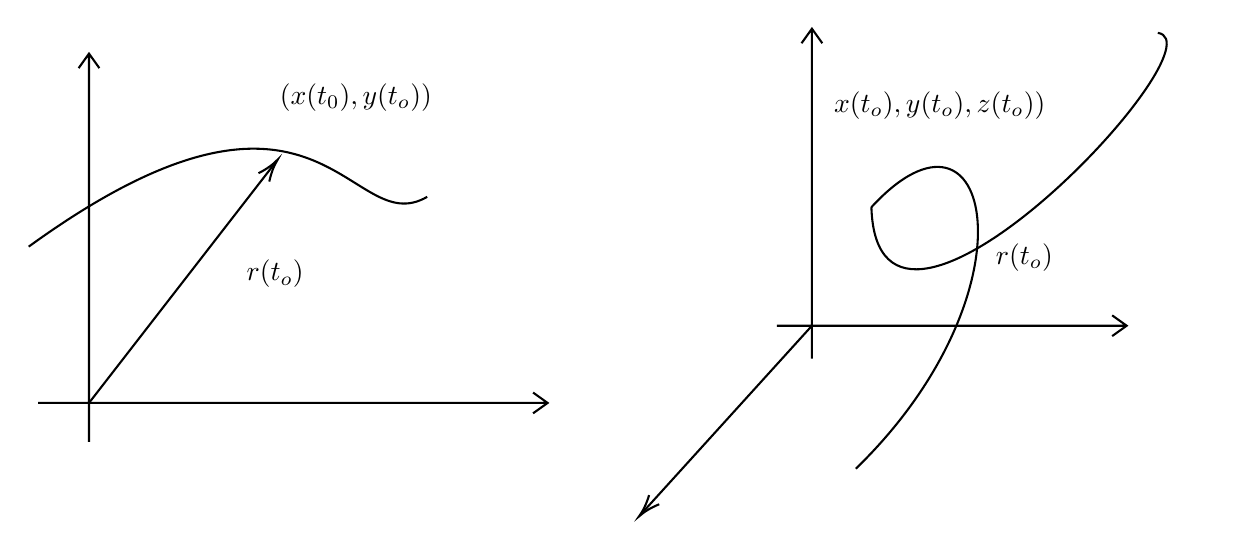
\begin{tikzpicture}[x=0.75pt,y=0.75pt,yscale=-1,xscale=1]
%uncomment if require: \path (0,310); %set diagram left start at 0, and has height of 310

%Shape: Axis 2D [id:dp34825501509521994] 
\draw  (23,212.3) -- (268.5,212.3)(47.55,44) -- (47.55,231) (261.5,207.3) -- (268.5,212.3) -- (261.5,217.3) (42.55,51) -- (47.55,44) -- (52.55,51)  ;
%Straight Lines [id:da7120917074211834] 
\draw    (47.55,212.3) -- (137.27,96.58) ;
\draw [shift={(138.5,95)}, rotate = 487.79] [color={rgb, 255:red, 0; green, 0; blue, 0 }  ][line width=0.75]    (10.93,-3.29) .. controls (6.95,-1.4) and (3.31,-0.3) .. (0,0) .. controls (3.31,0.3) and (6.95,1.4) .. (10.93,3.29)   ;
%Curve Lines [id:da9112376831548035] 
\draw    (18.5,137) .. controls (160.5,34) and (172.5,135) .. (210.5,113) ;
%Shape: Axis 2D [id:dp7523057169401708] 
\draw  (379,175.1) -- (547.5,175.1)(395.85,32) -- (395.85,191) (540.5,170.1) -- (547.5,175.1) -- (540.5,180.1) (390.85,39) -- (395.85,32) -- (400.85,39)  ;
%Straight Lines [id:da25097728151684107] 
\draw    (395.85,175.1) -- (313.84,265.52) ;
\draw [shift={(312.5,267)}, rotate = 312.21000000000004] [color={rgb, 255:red, 0; green, 0; blue, 0 }  ][line width=0.75]    (10.93,-3.29) .. controls (6.95,-1.4) and (3.31,-0.3) .. (0,0) .. controls (3.31,0.3) and (6.95,1.4) .. (10.93,3.29)   ;
%Curve Lines [id:da48745085294216717] 
\draw    (417,244) .. controls (505.5,158) and (482.5,55) .. (424.5,118) ;
%Curve Lines [id:da11758926162301764] 
\draw    (562.5,34) .. controls (595.5,39) and (427.5,217) .. (424.5,118) ;

% Text Node
\draw (138,57) node [anchor=north west][inner sep=0.75pt]    {$( x( t_{0}) ,y( t_{o}))$};
% Text Node
\draw (122,142) node [anchor=north west][inner sep=0.75pt]    {$r( t_{o})$};
% Text Node
\draw (405,61) node [anchor=north west][inner sep=0.75pt]    {$x( t_{o}) ,y( t_{o}) ,z( t_{o}))$};
% Text Node
\draw (483,134) node [anchor=north west][inner sep=0.75pt]    {$r( t_{o})$};


\end{tikzpicture}

\begin{definition}
\begin{align}
    \mi{x=f(t)&y=g(t)} a\leq t\leq b\\
    \mi{r(t)=\bv{f(t),g(t)}=f(t)\hat{i}+y(t)\hat{j}}\\
    \mi{r_o=\bv{x_o,x_o,z_o}&r_1=\bv{x_1,y_1,z_1}}\\
    \mi{t=(1-t)r_o+tr_1}
\end{align}
\end{definition}

\begin{exercise}
\begin{align}
    \intertext{¿Función vectorial? Para recta que va $P_o(3,2,-1)$ al punto $P_1(1,4,5)$}
    \mi{r(t)=(1-t)\bv{3,2,-1}+t\bv{1,4,5}}\\
    \mi{r(t)=\bv{3-2t,2+2t,-1+6t}}
\end{align}
\end{exercise}
%---
\begin{align}
    \mi{\vf{4\cos t}{+t}{+2\sin t}} &\text{c. helicoloides}
\end{align}
%---

\begin{align}
    \mi{\vf{t\cos t}{+t\sin t}{+t}}
\end{align}
%---
\begin{align}
    \mi{\vf{t^2}{+t^4}{+t^6}}
    \intertext{$x,y; y=x^3$ y $x,z; z=x^3$}
\end{align}

\subsection{Campos vectoriales}
\begin{definition}
\begin{align}
    \intertext{Sobre $\mathbf{R}^2$ una función $F$ que asigna a cada punto $(x,y)$ en $D$ (conjunto en $\mathbf{R}^2$) un vector bidimensional.}
    \mi{F(x,y)=\vfd{P(x,y)}{+Q(x,y)}}\\
    \mi{\bv{P(x,y),Q(x,y)}}\\
    \mi{F=P_i+Q_j}
    \intertext{También es posible expresarlas:}
    \mi{F(x,y,z)=\vf{P}{+Q}{+R}}
\end{align}
\end{definition}
%---
\begin{example}
\begin{align}
    \mi{F(x,y)=\vfd{-y}{+x}}\\
    \mi{||F||=C}\\
    \mi{\sqrt{y^2 +x^2}=C}
    \mi{x^2 +y^2 = C^2}\\
    \mi{(1,0)\mapsto\vfd{-(0)}{+(1)}=j}\\
    \mi{(0,1)\mapsto\vfd{-(1)}{+0}=-i}\\
    \mi{(1.5,1.5)\mapsto \vfd{-1.5}{+1.5}}
\end{align}
\end{example}
%---- 
\begin{example}
\begin{align}
    \mi{F(x,y)=\vfd{2x}{+y}}\\
    \mi{||F||=C}\\
    \mi{\sqrt{(2x)^2 +y^2}=C}\\
    \mi{4x^2 +y^2 =C^2 }& \text{elipse}\\
    \mi{(0.5,0)\implies 1i}\\
    \mi{(0,1)\implies 1j}\\
    \mi{(0.25,0.25)\implies \vfd{0.5}{+0.25}}\\
    \mi{(-2,-2)\implies \vfd{-4}{-2}}
\end{align}
\end{example}

%---- 
\begin{example}
\begin{align}
    \mi{F(x,y,z)=\vf{1}{-1}{0}}\\
    \mi{||F||=C}\\
    \mi{\sqrt{(1)^2 +(1)^2 +(0)^2}=\sqrt{2}}
\end{align}
\end{example}

\subsection{Gradiente}
\begin{definition}
\begin{align}
    \mi{f(x,y)=x^2 y+3xy^3}\\
    \mi{\nabla f(x,y)=\vfd{f_x(x,y)}{+f_y(x,y)})}\\
    \mi{\nabla f(x,y)=\vfd{(2xy+3y^3)}{+(x^2 +9xy^2)}}\\
    \intertext{Si $z=f(x,y)$}
\end{align}
\end{definition}

\begin{exercise}
\begin{align}
    \mi{f(x,y,z)=\sqrt{x^2+y^2+z^2}}\\
    \mi{\nabla(x,y,z)=\vf{\frac{x}{\sqrt{x^2 +y^2+z^2}}}{\frac{y}{\sqrt{x^2 +y^2+z^2}}}{\frac{z}{\sqrt{x^2 +y^2+z^2}}}}\\
\end{align}
\end{exercise}

\begin{exercise}
\begin{align}
    \intertext{Una partícula se mueve en un campo de velocidad $V(x,y)= \bv{x^2,x+y^2}$. Si su posición es (2,1) en un tiempo t=3, estime su posición en t=3.01}
    \mi{t=3\mapsto(2,1)}\\
    \mi{v(2,1)=\bv{2^2,2+1^2}=\bv{4,3}}\\
    \mi{t=3\mapsto3.01\implies0.001}\\
    \mi{0.01V(2,1)=0.01\bv{4,3}=\bv{0.04,0.03}}\\
    \mi{\text{Posición (2.04,1.03)}}
\end{align}
\end{exercise}
\subsection{Integral de Línea}
\begin{definition}
De $f$ a lo largo de $C$. 
\begin{align}
    \mi{\int_c f(x,y)ds = \lim_{n\mapsto\infty}}\suma{i=1}{n}{f(x_i^*,y_i^*)\Delta S}\\
    \intertext{$L=\ie{a}{b}{\sqrt{(\frac{dx}{dt})^2+(\frac{dy}{dt})^2}}{S}$}
    \mi{\int_c f(x,y)dS=\ie{a}{b}{f(x(t),y(t))*\sqrt{(\frac{dx}{dt})^2+(\frac{dy}{dt})^2}}{S}}
\end{align}
\end{definition}

\begin{exercise}
\begin{align}
    \mi{\ie{c}{}{(x^2-y+3z)}{S}}\\
    \intertext{x = t, y = 2t, z = t. En donde $0\leq t \leq$ }
    \intertext{x'=1,y=2,z=1.}
    \mi{\sqrt{(1)^2+(2)^2+(1)^2}=\sqrt{6}}\\
    \mi{\ie{c}{}{(x^2-y+3z)}{S}= \ie{0}{1}{(t^2 -2t +3t)\sqrt{6}}{t}}\\
    \mi{\sqrt{6}\ie{0}{1}{(t^2 +t)}{t}}\\
    \mi{\sqrt{6}[\frac{t^3}{3}+\frac{t^2}{2}]_0^1}\\
    \mi{=\frac{5\sqrt{6}}{6}}
\end{align}
\end{exercise}

\begin{exercise}
\begin{align}
    \mi{\ie{c}{}{(x+2)}{s}}
    \intertext{donde C es}
    \mi{r(t)=\vf{t}{+\frac{4t^{3/2}}{3}}{+\frac{t^2}{2}}}&0\leq t\leq 2\\
    \mi{||r'(t)||=\sqrt{(1)^2 +(2t^{1/2})^2+(t)^2}=\sqrt{1+4t+t^2}}\\
    \mi{\ie{c}{}{(x+2)}{s}=\ie{0}{2}{(t+2)\sqrt{1+4t+t^2}}{t}}\\
    \mi{=15.29}&x=t,y=\frac{4}{t^{2/2}},z=\frac{t^2}{2}
\end{align}
\end{exercise}


